%Documentation for FLUKE copyright 2014 Eric G. Kratz

\documentclass[12pt]{report}
\usepackage[hidelinks,bookmarks]{hyperref}
\usepackage[margin=1in]{geometry}
\usepackage{graphicx}
\usepackage{dtklogos}
\usepackage{amsmath,amssymb}
\usepackage{microtype}
\usepackage{placeins}
\usepackage{color}
\raggedbottom

\setlength\parindent{0cm}

\title{{\color{blue}FLUKE:} {\color{red}F}ields {\color{red}L}ayered 
{\color{red}U}nder {\color{red}K}ohn-Sham {\color{red}E}lectrons
\\ \vspace{3cm}
\begin{center}
\centering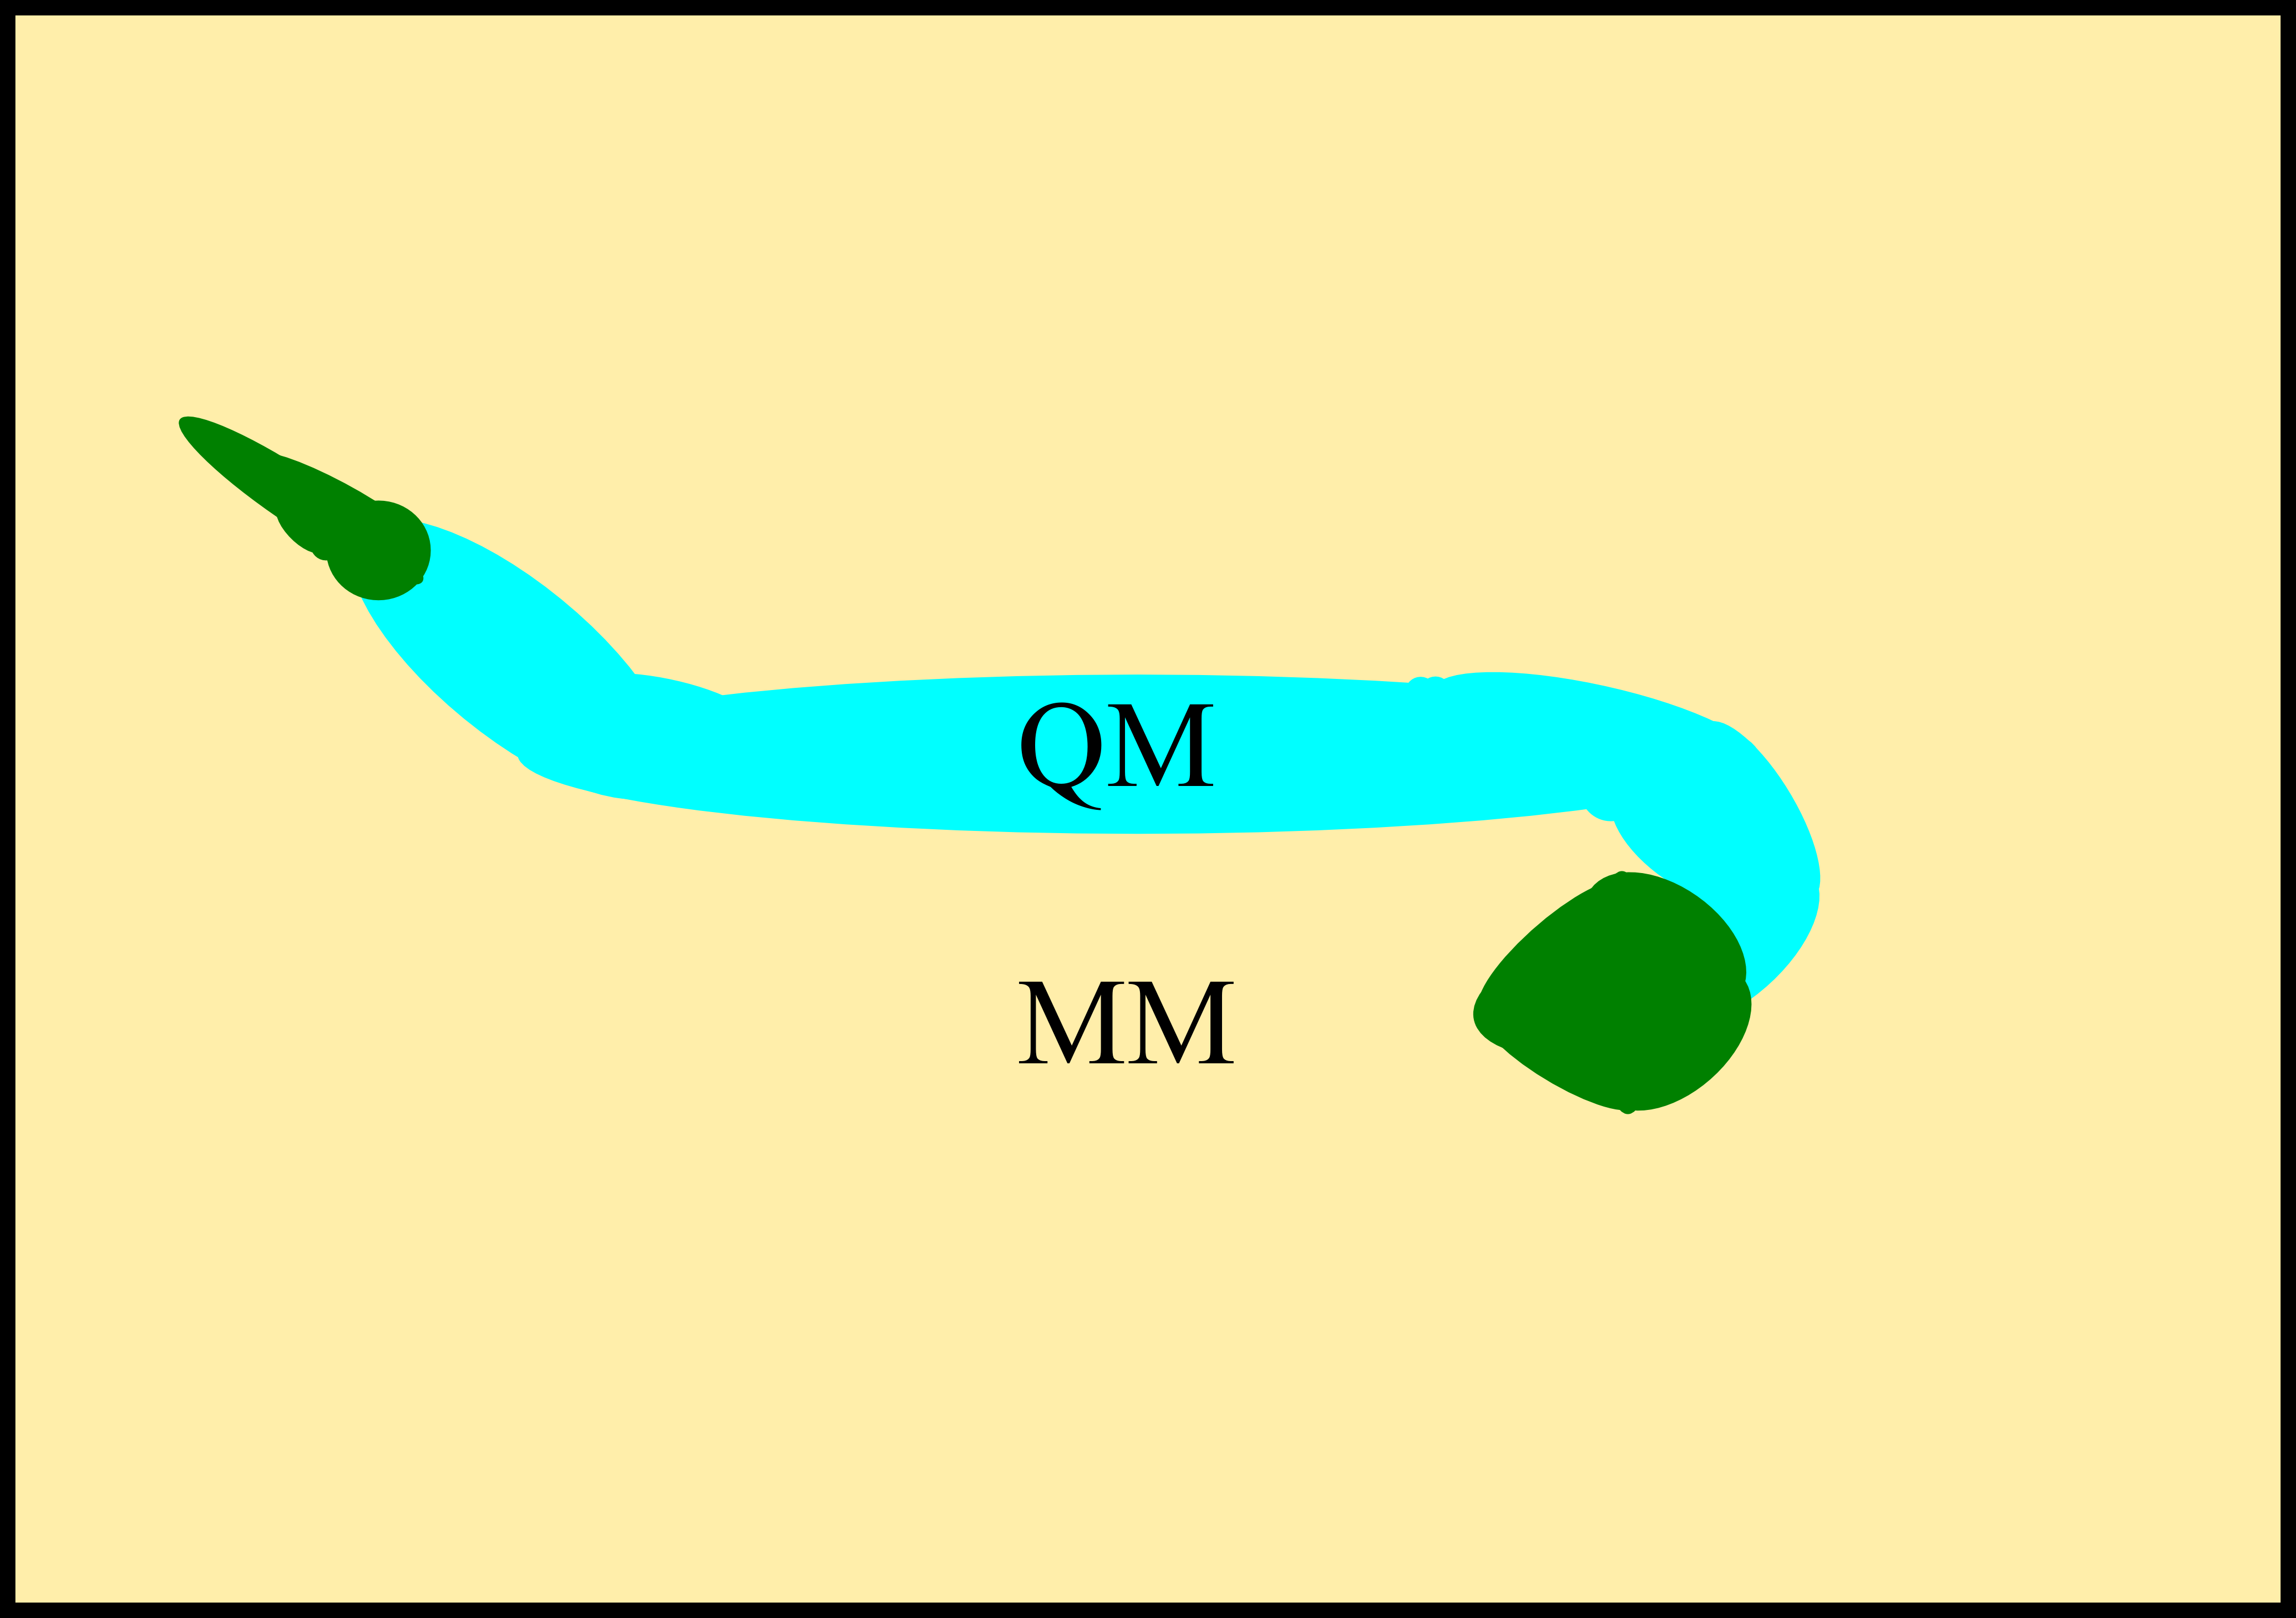
\includegraphics[scale=0.60]{../doc/images/QMMM_0.png}
\end{center}}
\author{A QMMM Interface for Polarizable Force Fields}
\date{Eric G. Kratz, 2014}

\begin{document}
\maketitle
\tableofcontents

\chapter{Introduction}

\section{Design Principles}

FLUKE is in development with four guiding principles: \\
\begin{quote}
 \normalfont{
 1) \textbf{FLUKE should primarily be an interface.} In order to make the
 code function with a variety of software packages and for different 
 versions of the packages, FLUKE should not require modifications to other
 software packages or tools. \\ 
 2) \textbf{FLUKE should be easy to read and modify.} Most scientists
 are not experts in computer programming. In order to allow for
 collaborative development of FLUKE, the source code needs to be easy
 to read. To that end, the code should be simple, well commented, and
 avoid linking to esoteric libraries. \\
 3) \textbf{FLUKE should be a single executable.} Since FLUKE is an
 interface, there is no need for a large collection of binaries. Having
 many different single-use executable files can discourage new users.
 Furthermore, FLUKE can be statically linked to ease distribution of the
 software. \\
 4) \textbf{FLUKE should be open source.} FLUKE is licensed under the GPLv3.
 Science can benefit everyone, and hence, should be shared as widely as
 possible. Additionally, I do  not want to see my effort in creating a large
 software package go to waste in a package that can only be used by a handful
 of scientists.}
\end{quote}

\section{Installation}

Since FLUKE is designed to be simple, only a small number of packages are
required to compile the code. An approximate list of packages is given
below.
\begin{quote}
 \normalfont{
 FLUKE binary: OpenMP, Eigen3 \\
 FLUKE manual: \LaTeX, \BibTeX}
\end{quote}

Clone the git repository or unpack FLUKE\_tarbomb.tgz \\

user:\$ mkdir FLUKE \\
user:\$ git clone https://github.com/kratman/FLUKE\_QMMM.git ./FLUKE/ \\

or \\

user:\$ mkdir FLUKE \\
user:\$ cd FLUKE/ \\
user:\$ tar -xvf FLUKE\_tarbomb.tgz \\

The FLUKE binary is included with the tgz source code, however, modified or
git versions can be compiled with the script provided with FLUKE. On Ubuntu
boxes, the compile script should function without modifications. However, with
other operating systems it may be necessary to change the path to the
\textit{Eigen3} package.

Default: -I/usr/include/eigen3/ \\

The compile script produces both the documentation and the source code.

user:\$ ./compile

\section{Capabilities}

\begin{table}[hbt]
 \centering
 \begin{tabular}{|c|c c|c c c|}
 \hline
  & Gaussian & PSI4 & TINKER & AMBER & LAMMPS \\ \hline
 QM energy & Yes & Yes & No & No & No \\
 MM energy & No & No & Yes & Yes & Yes \\
 QMMM energy & Yes & Yes & Yes & Yes & Yes \\ \hline
 QM opt. & Yes & Yes & No & No & No \\
 MM opt. & No & No & Yes & Yes & Yes \\
 QMMM opt. & Yes & No & Yes & Yes & Yes \\ \hline
 QM SD & Yes & Yes & No & No & No \\
 MM SD & No & No & No & No & No \\
 QMMM SD & Yes & Yes & Yes & Yes & Yes \\ \hline
 QM MC & Yes & Yes & No & No & No \\
 MM MC & No & No & Yes & Yes & Yes \\
 QMMM MC & Yes & Yes & Yes & Yes & Yes \\ \hline
 QM PIMC & Yes & Yes & No & No & No \\
 MM PIMC & No & No & Yes & Yes & Yes \\
 QMMM PIMC & Yes & Yes & Yes & Yes & Yes \\ \hline
 QM RP & Yes & No & No & No & No \\
 MM RP & No & No & No & No & No \\
 QMMM RP & Yes & No & Yes & Yes & Yes \\ \hline
 \end{tabular}
 \caption{Wrapper capabilities for single-point energy, geometry optimization,
 steepest descent (SD), Monte Carlo (MC), path-integral Monte Carlo (PIMC) and
 reaction path (RP) calculations.}
 \label{tab:WrapCap}
\end{table}

\subsection{QM and MM wrappers}

FLUKE can perform QM, MM, or QMMM calculations via an interface to packages
in the user's path. Temporary input files are created for each package and
the results are collected from the temporary output files. This is a
relatively inefficient procedure, however, reading and writing input/output
files is often negligible compared to the computational cost of the QM
calculation. Currently, calculations can be performed using Gaussian
\cite{Frisch2009}, PSI4 \cite{Turney2012}, TINKER \cite{}, AMBER \cite{}, and
LAMMPS \cite{Plimpton1995}. Additional wrappers can be added to FLUKE with
relatively little effort.

\subsection{Types of calculations}

Single-point energies, geometry optimizations, steepest descent minimizations
reaction pathways, classical Monte Carlo, and path-integral Monte Carlo
calculations can be performed using the QM and MM wrappers. Due to limitations
of the software packages, not all calculations can currently be performed with
all combinations of wrappers. For convenience, the capabilities are summarized
in Table \ref{tab:WrapCap}. \\

Some additional restrictions are also present when there are bonds between
the QM and MM regions. Currently only Gaussian can be used as a QM wrapper
for calculations where the QM and MM regions are bonded.

\FloatBarrier

\section{Acknowledgements}

The development of FLUKE was supported by funding from the NIH. FLUKE is
maintained by the Cisneros research group at Wayne State University.

\chapter{Input}

\section{Command line arguments}

FLUKE can only be invoked from a command line interface.

user:\$ FLUKE -n Ncpus -x xyzfile.xyz -c confile.inp
 -r regfile.inp -o output.xyz \\

-n: Number of CPUs used in the calculations. Note that during PIMC and
reaction path calculations each replica uses this many CPUs. A reaction
path calculation with 8 points and Ncpus=2 would require 16 CPUs. \\

-x: File name for the input structure in XYZ or PDB format. The XYZ input
should be in the standard format and have a blank comment line. \\

-c: File name for connectivity and force field information. \\

-r: File name for definitions of QMMM regions, QM wrapper, MM wrapper,
and general simulation options. \\

-o: File name for trajectories and optimized structures. \\

\section{XYZ input files}

The input structure for FLUKE is a standard XYZ file with a blank comment
line. \\

N \\

A  X$_A$  Y$_A$  Z$_A$ \\
B  X$_B$  Y$_B$  Z$_B$ \\
... \\

Here N is the number of atoms and (X$_i$,Y$_i$,Z$_i$) is the position of
particle $i$. Note that the atom types given in the XYZ file need to be the
atomic symbols from the periodic table, not the MM atom types. Additionally,
FLUKE reads the XYZ file item-by-item, which means that having additional
values on a line will cause (silent) errors.

\section{Connectivity input files}

The connectivity of the molecules and the force field information are defined
in the connectivity file. The general format is given below. \\

id MMTyp NumTyp q Nbonds [connectivity] \\
... \\

Here id is the index of the atom (0 to N-1), MMTyp is the force field atom
type (i.e. AMBER atom types), NumTyp is a numerical atom type (i.e. TINKER
atom types), q is the force field charge on the atom, Nbonds is the number of
bonds to the atom, and [connectivity] is the bond list . The length of the
connectivity list must match Nbonds and the information in the connectivity
file must be given for all atoms, even if there are no MM atoms in the system.
An additional caveat is that the atoms must be listed in order. This is part
of an internal check to make sure correct input files were provided.

\section{Region input files}

The region file contains QMMM regions (QM atoms, pseudo-atoms, boundary atoms,
and frozen atoms) as well as miscellaneous input needed to define the type
of calculations that will be performed. This is the most complicated input
file required by FLUKE and currently the input keywords must be given in the
correct order. The keywords themselves are only guides for making the files
human readable and only the values after the keywords are read. Blank templates
of region files are provided in the documentation directory.

The first line of the input file should read: \\

Potential\_type: $<$QM or MM or QMMM$>$ \\

This line tells FLUKE what type of QM and MM input is listed in the lines that
follow.

\subsection{General notes}

Input that is not specific to the wrappers is mostly case insensitive,
however, users may find exceptions to this rule of thumb. Future versions of
FLUKE will have a more robust input reader. In the mean-time, please report
any bugs that are found.

\subsection{QM input}

If the potential type is QM or QMMMM, several keywords are required to define
the QM wrapper and level of theory. \\

QM\_type: $<$Gaussian or PSI4$>$ \\
QM\_functional: $<$functional$>$ \\
QM\_basis: $<$basis set$>$ \\
QM\_memory: $<$RAM in GB$>$ \\
QM\_charge: $<$charge on the QM region$>$ \\
QM\_spin: $<$multiplicity of the QM region$>$ \\

All of the QM input is read into FLUKE as text, and hence, it must match the
correct input for the QM package. For example, Gaussian can only read integer
values for the memory.

\subsection{MM input}

If the potential type is MM or QMMM, several keywords are required to define
the MM wrapper. \\

MM\_type: $<$TINKER or AMBER or LAMMPS$>$ \\

All of the MM input is read into FLUKE as text, and hence, it must match the
correct input for the MM package.

\subsection{QMMM input}

QMMM input is a combination of the QM and MM input described above. \\

QM\_type: $<$Gaussian or PSI4$>$ \\
QM\_functional: $<$functional$>$ \\
QM\_basis: $<$basis set$>$ \\
QM\_memory: $<$RAM in GB$>$ \\
QM\_charge: $<$charge on the QM region$>$ \\
QM\_spin: $<$multiplicity of the QM region$>$ \\
MM\_type: $<$TINKER or AMBER or LAMMPS$>$ \\

All of the QMMM input is read into FLUKE as text, and hence, it must match the
correct input for the QM and MM packages. For example, Gaussian can only read
integer values for the memory.

\subsection{Simulation input}

Input for the calculation types directly follows the wrapper input. Each type
of calculation requires slightly different input. FLUKE can perform
single-point energies (SP), optimizations (Opt), and path-integral Monte Carlo
simulations (PIMC). Classical Monte Carlo simulations are performed as PIMC
simulations with a single bead. All calculation types are documented below. \\

Calculation\_type: $<$SP or Energy$>$ \\

Calculation\_type: Opt \\
Max\_opt\_step: $<$Size of the maximum optimization step (\AA)$>$ \\
MM\_opt\_tolerance: $<$Criteria to stop MM optimization$>$ \\
Max\_opt\_steps: $<$Run at most N QM steps per iteration$>$ \\

Calculation\_type: Steep \\
Opt\_step\_size: $<$Initial scale factor for the step size$>$ \\
Max\_opt\_step: $<$Size of the maximum optimization step (\AA)$>$
QM\_opt\_tolerance: $<$Criteria to stop the QM optimization$>$\\
MM\_opt\_tolerance: $<$Criteria to stop MM optimization$>$ \\
Max\_opt\_steps: $<$Run at most N QM steps per iteration$>$ \\

Calculation\_type: DFP \\
Opt\_step\_size: $<$Initial scale factor for the step size$>$ \\
Max\_opt\_step: $<$Size of the maximum optimization step (\AA)$>$
QM\_opt\_tolerance: $<$Criteria to stop the QM optimization$>$\\
MM\_opt\_tolerance: $<$Criteria to stop MM optimization$>$ \\
Max\_opt\_steps: $<$Run at most N QM steps per iteration$>$ \\

Calculation\_type: PIMC \\
Ensemble: $<$NVT or NPT$>$ \\
Temperature: $<$Temperature in Kelvin$>$ \\
Pressure: $<$Pressure in atm $>$ \\
Number\_of\_eq\_steps: $<$Run N steps before collecting data$>$ \\
Number\_of\_MC\_steps: $<$Collect data for N steps$>$ \\
Number\_of\_beads: $<$Number of PI beads$>$ \\
Acceptance\_ratio: $<$Fraction of attempted moves which succeed$>$ \\
Traj\_steps\_before\_printing: $<$Print every N steps$>$ \\

Calculation\_type: MD \\
Timestep: $<$Timestep in fs$>$ \\
Temperature: $<$Temperature in Kelvin$>$ \\
Number\_of\_eq\_steps: $<$Run N steps before collecting data$>$ \\
Number\_of\_MD\_steps: $<$Collect data for N steps$>$ \\
Traj\_steps\_before\_printing: $<$Print every N steps$>$ \\

\subsection{Region input}

Four different regions of the structure need to be defined even if the
regions contain zero atoms. \\

QM\_atoms: Nqm [list of ids] \\
Pseudo\_atoms: Npseudo [list of ids] \\
Boundary\_atoms: Nbound [list of ids] \\
Frozen\_atoms: Ninact [list of ids] \\

Definitions of the QM, pseudo-atoms, and boundary atoms can be found in
Chapter \ref{chap:Theory}. Frozen atoms are atoms that should remain
stationary during optimizations or Monte Carlo simulations. Frozen atoms are
useful for optimizing small regions of large periodic systems. \\

Note that in pure QM and pure MM simulations, \{Nqm,Npseudo,Nbound\} can all
be set to zero. This is because these regions are not relevant unless FLUKE is
performing a QMMM calculation. For all of the regions, the lists of atoms can
be separated by either spaces or newlines.

\section{Input generation}

While FLUKE does not handle atom typing or structure generation, it is
possible to use the native input/output functions to create FLUKE input from
input used for MM packages. In all cases the converter produces three
files: xyzfile.xyz connect.inp regions.inp \\

TINKER: The file converter for TINKER can be used on standard
TINKER XYZ files, TINKER QMMM XYZ files (Q-CHEM), and TINKER XYZ files
with periodic boundary conditions. \\

user:\$ FLUKE -convert -t TINKER.xyz -k tinker.key ( -p Yes) \\

The -p flag is optional and tells FLUKE to read the lattice constants from
the second line of the XYZ file. \\

AMBER: \\

LAMMPS:

\section{FLUKE output}

Most of the FLUKE output is sent through the c++ std output stream. However,
trajectories and optimized structures are printed into the file defined
by the -o flag. In single-point energy calculations, the output XYZ file
is deleted after the calculation is completed, since the geometry does not
change during the calculation.

\section{Additional input for wrappers}

The FLUKE wrappers automatically look for a couple "extra" input files. These
files depend on which wrappers are used in the calculation, however, in most
cases the files contain force field and pseudopotential information. Some of
the extra files are detailed below in no particular order and examples can be
found in the documentation directory.

\subsection{TINKER}

The TINKER wrapper checks the working directory for a file called tinker.key
and will read additional force field information (e.g. atom classes,
multipoles, etc) based on the keywords listed in that file. Any keyword
defined in tinker.key will be passed into the TINKER key file used by the
wrapper. For somewhat obvious reasons, the user must also provide the force
field parameter files defined in the tinker.key file.

\subsection{Gaussian}

The Gaussian wrapper will look for a file called BASIS in the working
directory. This file contains basis and pseudopotential information for
QMMM calculations with bonds between the QM and MM regions (see below).
While the file is read in automatically if it is found, the user still needs
to tell Gaussian to use this information: \\

QM\_basis: GEN \\

GEN is a Gaussian keyword which causes the package to check for extra basis
set information below the structure. \\

FLUKE automatically tells Gaussian to look for pseudo potentials, however,
these must be given below the basis set information in the BASIS file. Both
the basis set and pseudopotential information must be given in Gaussian
format.

\chapter{Theoretical Background}
\label{chap:Theory}

\section{Preface}

The following chapter is intended to serve as a general introduction to
computational chemistry and the methods used in FLUKE. There are numerous
places users can find more detailed and up-to-date discussions of these
topics. This chapter is only intended to give a broad review of the concepts
and terminology.

\section{Classical Methods}

\subsection{Newton's laws of motion}

Much of classical physics can be described in terms of Newton's three laws of
motion.
\begin{quote} 
 \normalfont{
 1) An object in motion tends to stay in motion unless it is acted upon by a
 force. \\
 2) The force on an object is equal to its mass times its acceleration
 ($F=ma$). \\
 3) For every action, there is an equal and opposite reaction.}
\end{quote}
Newton's second law can be employed in calculations to predict the position
and velocity of objects moving in a potential field. A simplified algorithm
for the discretized equations of motion can be written as
\begin{equation}
 F_{n} = -\nabla V_{n} = m\ddot r_{n} \; ,
\end{equation}
\begin{equation}
 \dot r_{n+1} = \dot r_{n}+\ddot r_{n}\Delta t \; ,
\end{equation}
and
\begin{equation}
 r_{n+1} = r_{n}+\dot r_{n}\Delta t+\frac{\ddot r_{n}\Delta t^2}{2} \; ,
\end{equation}
where $F$ is the force, $V$ is the potential energy, $r$ is a vector
representing the positions of all atoms in the system, and $\Delta t$ is the
time interval between time step $n$ and $n+1$. The natural ensemble for
molecular dynamics is the microcanonical ensemble (NVE), where the number of
particles and energy are conserved inside a constant volume simulation box.
Although the NVE simulations are the native result of propagating Newton's
equations, most experiments are performed in the canonical (NVT) or
isothermal-isobaric (NPT) ensembles. In the NVT ensemble, the temperature is
held constant instead of the energy, and the NPT ensemble also holds the
pressure to be constant by adjusting the size of the simulation box.

\subsection{Force fields}

Empirical force fields are classical potentials which can estimate the
potential energy of a system. Although any functional form could be employed
for the force field, the potentials are often derived from experiments,
classical physics, or quantum theory. \\

Non-bonded interactions of atoms are typically modeled using point-charges
and Lennard-Jones potentials or other van der Waals potentials. The non-bonded
potential is given by
\begin{equation}
 V(R) = V_{coul}(R)+V_{vdW}(R) \; ,
\end{equation} 
\begin{equation}
 V_{coul}(R) = C\sum \frac{q_iq_j}{r_{ij}} \; ,
\end{equation}
and
\begin{equation}
 V_{vdW}(R) = \sum \frac{A_{ij}}{r_{ij}^{12}}
              -\frac{B_{ij}}{r_{ij}^{6}} \; ,
\end{equation}
where $R$ is a vector representing the coordinates of the system, $V(R)$ is the
potential, $V_{coul}(R)$ is the Coulomb potential for point-charges ($q$),
$C$ is a constant, $r_{ij}$ is the distance between atoms $i$ and $j$,
$V_{vdW}(R)$ is the van der Waals potential (in this case, the Lennard-Jones
potential), $A_{ij}$ is a parameter representing the exchange interaction, and
$B_{ij}$ is a parameter representing the dispersion interaction. \\

Bonded interactions are often represented by the harmonic potential. Harmonic
bonds behave as idealized springs that never weaken or break. The harmonic
potential is given by
\begin{equation}
 V_{harm}(r_{ij}) = \frac{K_{ij}}{2}r_{ij}^2 \; ,
\end{equation}
where $K_{ij}$ is the spring constant. Similarly, bond angles can be described
by a harmonic potential
\begin{equation}
 V_{harm}(\theta_{ijk}) = \frac{K_{ijk}}{2}\theta_{ijk}^2 \; ,
\end{equation}
where $\theta$ is the angle between atoms $i$, $j$, and $k$. More complicated
potentials can be constructed for the bonded interactions, but these are two
of the most common potentials. Typically, large molecules require potentials
for dihedral angles and improper dihedral angles. \\

The parameters for force fields are determined in a very systematic fashion.
Typically, the charges are determined from electronic structure calculations
and bonded parameters are determined by matching the molecular vibrational
modes. The van der Waals parameters are usually adjusted to reproduce
the density, enthalpy of freezing, or other experimentally determined
properties.

\subsection{Polarizable force fields}

Point-charges are often inadequate for representing the electrostatic field
around a molecule. The field can be improved by assigning point-charges ($q$),
dipoles ($\mu$), quadrupoles ($\Theta$), and polarizabilities ($\alpha$) to
the atoms. These force fields are more computationally expensive than standard
point-charge force fields, however, the results can be much more accurate.

A Cartesian representation of the multipoles can be simplified by converting
to a spherical harmonic representation. The first step in the conversion is to
diagonalize the quadrupole tensor
\begin{equation}
 R^{-1}\Theta R = \Theta' \; ,
\end{equation}
where $R$ are the eigenvectors and $\Theta'$ are the eigenvalues. The
Cartesian multipoles through the quadrupole moments can be converted to the
spherical harmonic multipoles, $Q$
\begin{equation}
 Q_{00} = q \; ,
\end{equation}
\begin{equation}
 Q_{11c} = \vec \mu \cdot R_x \; ,
\end{equation}
\begin{equation}
 Q_{11s} = \vec \mu \cdot R_y \; ,
\end{equation}
\begin{equation}
 Q_{10} = \vec \mu \cdot R_z \; ,
\end{equation}
\begin{equation}
 Q_{22c} = (\Theta_{xx}-\Theta_{yy})/\sqrt{3} \; ,
\end{equation}
\begin{equation}
 Q_{20} = \Theta_{zz} \; ,
\end{equation}
where $R_i$ are the eigenvectors in the $i$ direction. The spherical harmonic
representation reduces the the multipole expansion to six moments in the new
frame of reference defined by $R$. \cite{} \\

The spherical harmonic multipole expansion through quadrupole moments can be
converted to six point-charges. \cite{}
\begin{equation}
 q_{\pm x} = \frac{Q_{00}}{6} \pm \frac{Q_{11c}}{2d} -
          \frac{Q_{20}}{6d^2} + \frac{Q_{22c}}{2\sqrt{3}d^2} \; ,
\end{equation}
\begin{equation}
 q_{\pm y} = \frac{Q_{00}}{6} \pm \frac{Q_{11s}}{2d} -
          \frac{Q_{20}}{6d^2} - \frac{Q_{22c}}{2\sqrt{3}d^2} \; ,
\end{equation}
\begin{equation}
 q_{\pm z} = \frac{Q_{00}}{6} \pm \frac{Q_{10}}{2d} +
          \frac{Q_{20}}{3d^2} \; ,
\end{equation}
where $q_{\pm i}$ are the charges in the $\pm i$ direction, and $d$ is the
displacement from the atomic center. While representing the multipoles as a
set of point-charges reduces the accuracy, most QM and MM packages can easily
add additional point-charges to the potential.

\subsection{Frozen density force fields}

Frozen density force fields are a special class of polarizable force fields
where the electron density is represented by Gaussian functions. These
potentials can greatly improve the calculations of the electrostatic field and
can include exchange and charge penetration effects.

\FloatBarrier

\section{Quantum Methods}

\subsection{Schr\"{o}dinger equation}

Quantum behavior can be described using the Schr\"{o}dinger wave equation and
the Hamiltonian operator, $\hat H$,
\begin{equation}
 \hat H = \hat T + \hat V \; ,
\end{equation}
where $\hat T$ is the kinetic energy operator and $\hat V$ is the potential
energy operator. The Schr\"{o}dinger equation is given by
\begin{equation}
 \hat H\psi = E\psi \to E = \int \psi^*\hat H\psi d\tau \; ,
\end{equation}
where $\psi$ is the wave function, $E$ is the energy, $^*$ denotes the complex
conjugate, and $\int d\tau$ is the integral over all space. The
Schr\"{o}dinger equation can also be written in terms of a determinant,
\begin{equation}
 |H-ES| = 0 \; ,
\end{equation}
where $S$ is the overlap matrix. Another common shorthand is bra-ket notation.
\begin{equation}
 \hat H|\psi\rangle = E|\psi\rangle \to E=\langle\psi|\hat H|\psi\rangle \; ,
\end{equation}
where $\langle i|\hat O|j\rangle$ is the integral of operator $\hat O$ on
state $j$.

\subsection{Perturbation theory}

If there is a complicated system and we want to solve the Schr\"{o}dinger 
equation, a good starting point is often to use a system for which the exact
solution is known. In chemistry, this is often the hydrogen atom, and in solid
state physics, it is often the "homogeneous electron gas". For example, helium
can be approximated as two electrons interacting with a nucleus, but not with
each other (i.e. solving the hydrogen problem twice with a nuclear charge of
+2). \\

Mathematically, the Hamiltonian can be divided into the simple parts and the
ones we wish we did not have to solve,
\begin{equation}
 \hat H = \hat H_0+\hat H_1+\hat H_2+\cdots \; ,
\end{equation}
where $\hat H$ is the full Hamiltonian, $\hat H_0$ is the simple
(zeroith-order) Hamiltonian that we can solve analytically, and $\hat H_i$
($i$=1,2...) are the $i$th-order Hamiltonians for interactions that have been
neglected in $\hat H_0$. The Schr\"{o}dinger equation can then solved for the
simple system,
\begin{equation}
 \hat H_0\psi_0=E_0\psi_0 \; .
\end{equation}

Perturbation theory adds the $i$th-order Hamiltonians to the zeroth-order
energy as the average interactions (based on the probability from the
wave function). This is easiest to understand for first-order perturbation
theory, however, the higher-order corrections are systematic and
straightforward. The perturbed Schr\"{o}dinger equation is given as
\begin{equation}
 \hat H\psi=E\psi \to (\hat H_0 + \hat H_1)\psi = E\psi \; , 
\end{equation}
and
\begin{equation}
 E \approx E_0 + E_1 \approx E_0 + \langle\psi_0|\hat H_1|\psi_0\rangle \; .
\end{equation}

Note that first-order perturbation theory uses the zeroth-order wave 
function for the averages. This can be seen as both an advantage and a
disadvantage in the calculations. The advantage is that it speeds up the
calculation to use a lower-order wave function since the higher order terms
have no effect on the solution of the simpler system. The disadvantage is that
wave function itself does not respond to the higher-order interactions. For
helium with a first-order perturbation, the electrons are too close to the
nucleus since there is a strong nuclear attraction with no repulsion due to
the second electron. \\

It should be noted that perturbation theory can correct both the wave function
and the energy. However, the corrections to the wave function can be two orders
lower than the corrections to the energy. A third-order correction to the
energy would require a first-order correction to the wave function.

\subsection{Variational theorem}

Another method for solving the Schr\"{o}dinger equation involves approximating
the wave function for a complex system. If the Hamiltonian for a system is
known, but not the wave function, we can often make an educated guess. Since
the ground-state of a system is the one with the lowest energy, any
guess-wave function, $\phi$, must have an energy that is greater-than or
equal-to the ground-state energy. If the energy calculated using $\phi$ is
equal-to the true ground-state energy, then $\phi$ is the true ground-state
wave function. If $\hat H\phi=E\phi$ predicts an energy lower than the
ground-state energy, then the ground-state is not the lowest energy state
(impossible by definition). This theorem can be proven mathematically,
however, it is conceptually intuitive. \\

While the variational theorem may sound useful since a reasonable guess
wave function must be provided, we can often employ the properties of linear
combinations and the solutions of $\hat H_0\psi_0=E_0\psi_0$. When solving
differential equations, any linear combination of the solutions to the
equation is also a solution. For example, the 1s ground-state of the hydrogen
atom is a solution of the Schr\"{o}dinger equation for the hydrogen atom. The
2s excited state is another solution. Therefore,
\begin{equation}
 \phi = c_1\psi_{1s}+c_2\psi_{2s} \; ,
\end{equation}
is also a solution for the hydrogen atom. We call this a linear combination of
atomic orbitals (LCAO) wave function.

\subsection{Basis sets}

In principle, any set of functions (a basis set) can be chosen as a guess and
then the linear combination coefficients ($c_1$ and $c_2$ above) can be
adjusted to lower the energy. The more functions that are included in the
basis set, the closer the guess-wave function can get to the true wave
function of the system. A logical choice would be to use hydrogen-like wave
functions for the individual atoms in a molecule as the basis set, however,
the integrals are not easy to calculate. \\

A more practical solution is to choose a large set of functions that we can
easily integrate. For instance, Gaussian functions have great properties that
simplify integration. The STO-3G basis set provides a good example of how this
is done. A Slater-type orbital (STO) is a systematic hydrogen-like orbital for
any atomic state. The STO-3G basis set represents the STOs of the atoms as the
combination of 3 Gaussian functions. This produces approximate "hydrogen-like"
orbitals that have still have the mathematical properties of Gaussians. For
the hydrogen molecule, the wave function would be given by
\begin{equation}
 \psi \approx c_a\phi_{a,1s}+c_b\phi_{b,1s} \; ,
\end{equation}
where $\phi_{a,1s}$ and $\phi_{b,1s}$ are the 1s orbitals on the first and
second hydrogen atom, respectively. If $\phi_n$ is represented by the STO-3G
basis set, the wavefunciton is given by
\begin{equation}
 \psi \approx c_a(G^a_1+G^a_2+G^a_3)+c_b(G^b_1+G^b_2+G^b_3) \; ,
\end{equation}
where $G^j_i$ is the $i$th Gaussian functions centered on atom $j$. This
approximation produces a lot of Gaussian integrals, but only has two
coefficients that can be changed to lower the energy. Hence, the basis set has
two relatively easy to integrate orbitals made of three Gaussians each. \\

Next, let's consider the Pople basis sets which are written as w-xyzG. This
notation indicates how many Gaussians are used to represent the atomic
orbitals. For now, we can just use the lithium atom as the example for the
wave function,
\begin{equation}
 \psi = c_1\phi_{1s} + c_2\phi_{2s} + c_3\phi_{2p,x} +
 c_4\phi_{2p,y} + c_5\phi_{2p,z} \; .
\end{equation}
Lithium has five orbitals and five variational coefficients if we consider
$\phi_n$ to be an STO, but we are going to use more complicated basis sets. \\

The w in w-xyzG represents the number of Gaussian functions used to represent
the core orbitals (filled inner shells) and (x,y,z) represent the number of
Gaussian functions in the valence orbitals. For the moment let's ignore the p
orbitals ($\psi'$) and consider the 3-21G basis set (w=3,x=2,y=1,z=0) for the
s orbitals.
\begin{equation}
 \psi' = c_{1w}(G_1+G_2+G_3)+c_{2x}(G_4+G_5)+c_{2y}G_6 \; .
\end{equation}
The first three Gaussian functions represent the 1s orbital and have a single
variational coefficient. The second three Gaussians split the valence orbital
into a two Gaussian and one Gaussian function with two additional variational
parameters. These split valence basis sets are more flexible and perform
better compared to the STO valence states. The full 3-21G basis set for
lithium has nine variational parameters and a total of fifteen Gaussian
functions. The larger 6-311G basis set splits the valence states into three
parts (thirteen variational parameters, twenty total Gaussian functions). The
number of "parts" representing the valence orbitals is referred to as the zeta
level of the basis set. A single zeta basis set has one variational parameter
per valence orbital (e.g. STO-3G), a double zeta basis set has two variational
parameters per valence orbital (e.g. 6-31G), and a triple zeta basis set has
three parameters per valence orbital (e.g. 6-311G). \\

The Pople basis sets are often used with polarization and/or diffuse Gaussian
functions. Polarization functions are additional p, d, f, etc.\ orbitals on
top of the standard functions. The 6-31G(d) basis set adds d orbitals to the
heavy atoms (i.e. not hydrogen) and 6-31G(d,p) also adds p orbitals to the
hydrogens. This can be made much more complicated (i.e. 6-31G(df,pd)) but the
notation is straight-forward. There is also an older notation for the
polarization functions using * instead of the orbitals (6-31G*=6-31G(d) and
6-31G**=6-31G(d,p)). Diffuse functions are very large s orbitals (e.g. 5s, 6s)
added to the atomic basis sets. The notation is 6-31+G and 6-31++G for adding
diffuse functions to the heavy atoms and all atoms respectively. The
polarization and diffuse functions are often vital for small molecules, but
can be problematic in large systems. \\

Dunning basis sets have a simpler notation, but are mathematically much more
complicated. The notation is cc-pVnZ, where n is the zeta level. The notation
stands for "correlation consistent polarized valence n zeta" with
n=D,T,Q,5,6,etc. A cc-pVDZ basis set is approximately the same as the
6-31G(d,p) basis set. Diffuse functions are added to all atoms with aug-
(augmented), i.e. aug-cc-pVnZ. The Dunning basis sets are designed to
systematically converge to the infinite basis set, however, they are much more
computationally demanding than the Pople basis sets.

\subsection{Pseudopotentials}

Large or complicated systems can be simplified by discarding core electrons
and modifying the electron-nuclei interactions for the valence states. A
simple (albeit extremely inaccurate) example would be to combine the core
electrons of an atom with the nucleus (e.g. oxygen would have a nuclear charge
of six and four valence electrons). The modified potentials are referred to as
pseudopotentials. Pseudopotentials are useful for a variety of reasons, they
reduce the number of electrons, the least important electrons are removed,
basis functions have a difficult time modeling the core region, and they can
be designed to include relativistic effects. \\

Real pseudopotentials do not change the nuclear charge, but rather add an
electrostatic potential with the same spatial distribution as the electrons
they replace. A further advantage of pseudopotentials, which is employed in
QMMM calculations, is that the potentials can replace entire atoms. For
instance, a methyl group can be modeled as a fluorine atom combined with a
pseudopotential.

\subsection{Orbital-free density functional theory}

Density functional theory (DFT) is an elegant solution to problems in quantum
theory and is distinct from the other formalisms (matrix mechanics
(Heisenberg), wave mechanics (Schr\"{o}dinger), and the path-integral approach
(Feynman)). The idea is that you do not need to know the wave function, only
the electron density of the system, to calculate the energy. It can be proven
that there is a one-to-one relationship between a given electron density and
the energy of the system. This greatly simplifies the problem the problem
since electrons contribute three degrees of freedom (each) to the
Schr\"{o}dinger equation, while the density, $\rho$, always has a total of
three degrees of freedom.
\begin{equation}
 \hat H\psi=E\psi \to E[\rho] = T[\rho]+V[\rho] \; .
\end{equation}

DFT, in its original construction, does not require orbitals or basis sets.
The entire problem can be solved as a function of $\rho(x,y,z)$.
Unfortunately, the exact functional $E[\rho]$ is unknown and the functional
must be approximated. Functionals are often based on the homogeneous electron
gas, and the nuclei are treated as an external field which perturbs the
electrons. Current functionals are only approximate, however, they often
provide a computationally efficient solution for large systems. \\

The earliest orbital-free DFT functional was the Thomas-Fermi (TF) model,
\begin{equation}
 T[\rho(\textbf{r})] = C_{tf}\int \rho(\textbf{r})^{5/3}d\textbf{r} \; ,
\end{equation}
\begin{equation}
 V[\rho(\textbf{r})] = \int
 \frac{\rho(\textbf{r})\rho(\textbf{r}')}{2|\textbf{r}-\textbf{r}'|}
 d\textbf{r}d\textbf{r}'
 -\sum \int \frac{\rho(\textbf{r})Z_i}{|\textbf{r}-\textbf{r}_i|} d\textbf{r}
 \; ,
\end{equation}
and
\begin{equation}
 E[\rho(\textbf{r})] = T[\rho(\textbf{r})]+V[\rho(\textbf{r})] \; .
\end{equation}
Here $\textbf{r}$ is the position of an electron, $Z_i$ is the nuclear charge
of atom $i$, $\textbf{r}_i$ is the position of nucleus $i$, and $\textbf{r}'$
is the position of the second electron. This model only requires an
approximation for the electron density and the positions of the nuclei, and
hence, the electron density can be treated as a fluid instead of discrete
particles. \\

In general the electron-electron and electron-nucleus parts of the functional
are much more accurate than the kinetic energy functional. In fact, the one of
the simplest potential functionals (LDA) is still used, but the simplest
kinetic energy functional (TF) cannot even predict chemical bonding. A more
accurate approximation for the kinetic energy is discussed below.

\subsection{Self-consistent field methods}

The self-consistent field (SCF) or Hartee-Fock (HF) formalism takes advantage
of the topics discussed above to find a simple but relatively accurate
solution to the Schr\"{o}dinger equation. The method iteratively solves the
equations using the Fock operator, $F$,
\begin{equation}
 E = \langle\phi|\hat F|\phi\rangle \; ,
\end{equation}
\begin{equation}
 \hat F = \hat H_0+\langle\phi|\hat H_1|\phi\rangle \; ,
\end{equation}
until the variational wave function no-longer changes. The problem converges
since the Fock operator depends on the average electron-electron repulsion
from the previous iteration. The result is an approximate first-order energy
and a first-order wave function. \\

The HF method can be improved by adding additional perturbations. A
second-order correction to the HF energy is referred to as MP2, and up to
MP4 are often discussed in the literature. The MP2 energy, $E_{mp2}$, is
given by
\begin{equation}
 E_{mp2} = E_{hf} + \langle E_{2} \rangle \; ,
\end{equation}
where $E_{hf}$ is the HF energy and $\langle E_2 \rangle$ is the second-order
perturbation. \\

There is a bit of terminology that has thus far been missing from the
discussions. The first is "electron correlation", which refers to the
interactions and motions of the electrons (i.e. an electron wants to move away
from another electron). In the literature, the "correlation energy" is
the electron-electron interaction energy not captured by the HF method
(second-order and higher perturbations). The SCF formalism is only a
mean-field approach, and hence, it gives the average interactions not the true
interactions. The second bit of terminology is the "exchange interaction",
which is included in $\hat F$ through $\hat H_1$. The solution of the
Schr\"{o}dinger equation for electrons should be anti-symmetric with respects
to the exchange of two electrons. The exchange interaction is added to the
$\hat H_1$ operator to force the variational wave function to have the correct
symmetry. \\

Hartree-Fock calculations capture the exchange, but miss the higher-order
correlation. Density functional theory calculations, on the other hand,
capture some of the higher-order correlation, but miss some of the exchange
interaction.

\subsection{Kohn-Sham DFT}

Kohn-Sham (KS) DFT is a SCF approach similar to HF theory, however, it does
not obey the variational theorem. To overcome the failures of the orbital-free
kinetic energy functionals, orbitals are reintroduced to the problem so that
the kinetic energy can be calculated "exactly" from a basis set. As with the
HF method, the electrons are moving in a mean-field of all other electrons,
but are not interacting directly. Since KS-DFT has orbitals, the exchange
interaction can also be calculated "exactly" with only a modest increase in
computational cost. However, since most functionals include an exchange term,
hybrid functionals add in a percentage of the exact (HF level) exchange and
remove the same percentage of DFT exchange. Researchers can make entire
careers out of developing better functionals (there are currently thousands)
and the mathematical structure of the functionals can be quite complicated.
However, some of the most common functionals are LDA (based on the electron
gas, used in solid state physics), PBE (contains no empirical parameters, used
in physics), PBE0 (a hybrid form of PBE with 25\% HF exchange, used in
physics), and B3LYP (a hybrid functional with three empirical parameters, used
heavily by chemists).

\subsection{Dispersion corrections}

KS-DFT does a reasonably good job for describing bonded interactions, metals,
geometries, and energies. However, DFT poorly describes van der Waals
interactions, such as dispersion. Modern functionals are often dispersion
corrected by adding empirical corrections to the nuclei-nuclei interactions.
For the most part, the dispersion energy, $E_d$, takes the form
\begin{equation}
 E_d = \sum_{i,j} f(R_{ij})\frac{C_6}{R_{ij}^6} \; ,
\end{equation}
where $C_6$ is an emprical parameter, $f(R_{ij})$ is a damping function, and
$R_{ij}$ is the distance between atoms $i$ and $j$.

\FloatBarrier

\section{QMMM}

\begin{figure}[hbt]
 \centering
 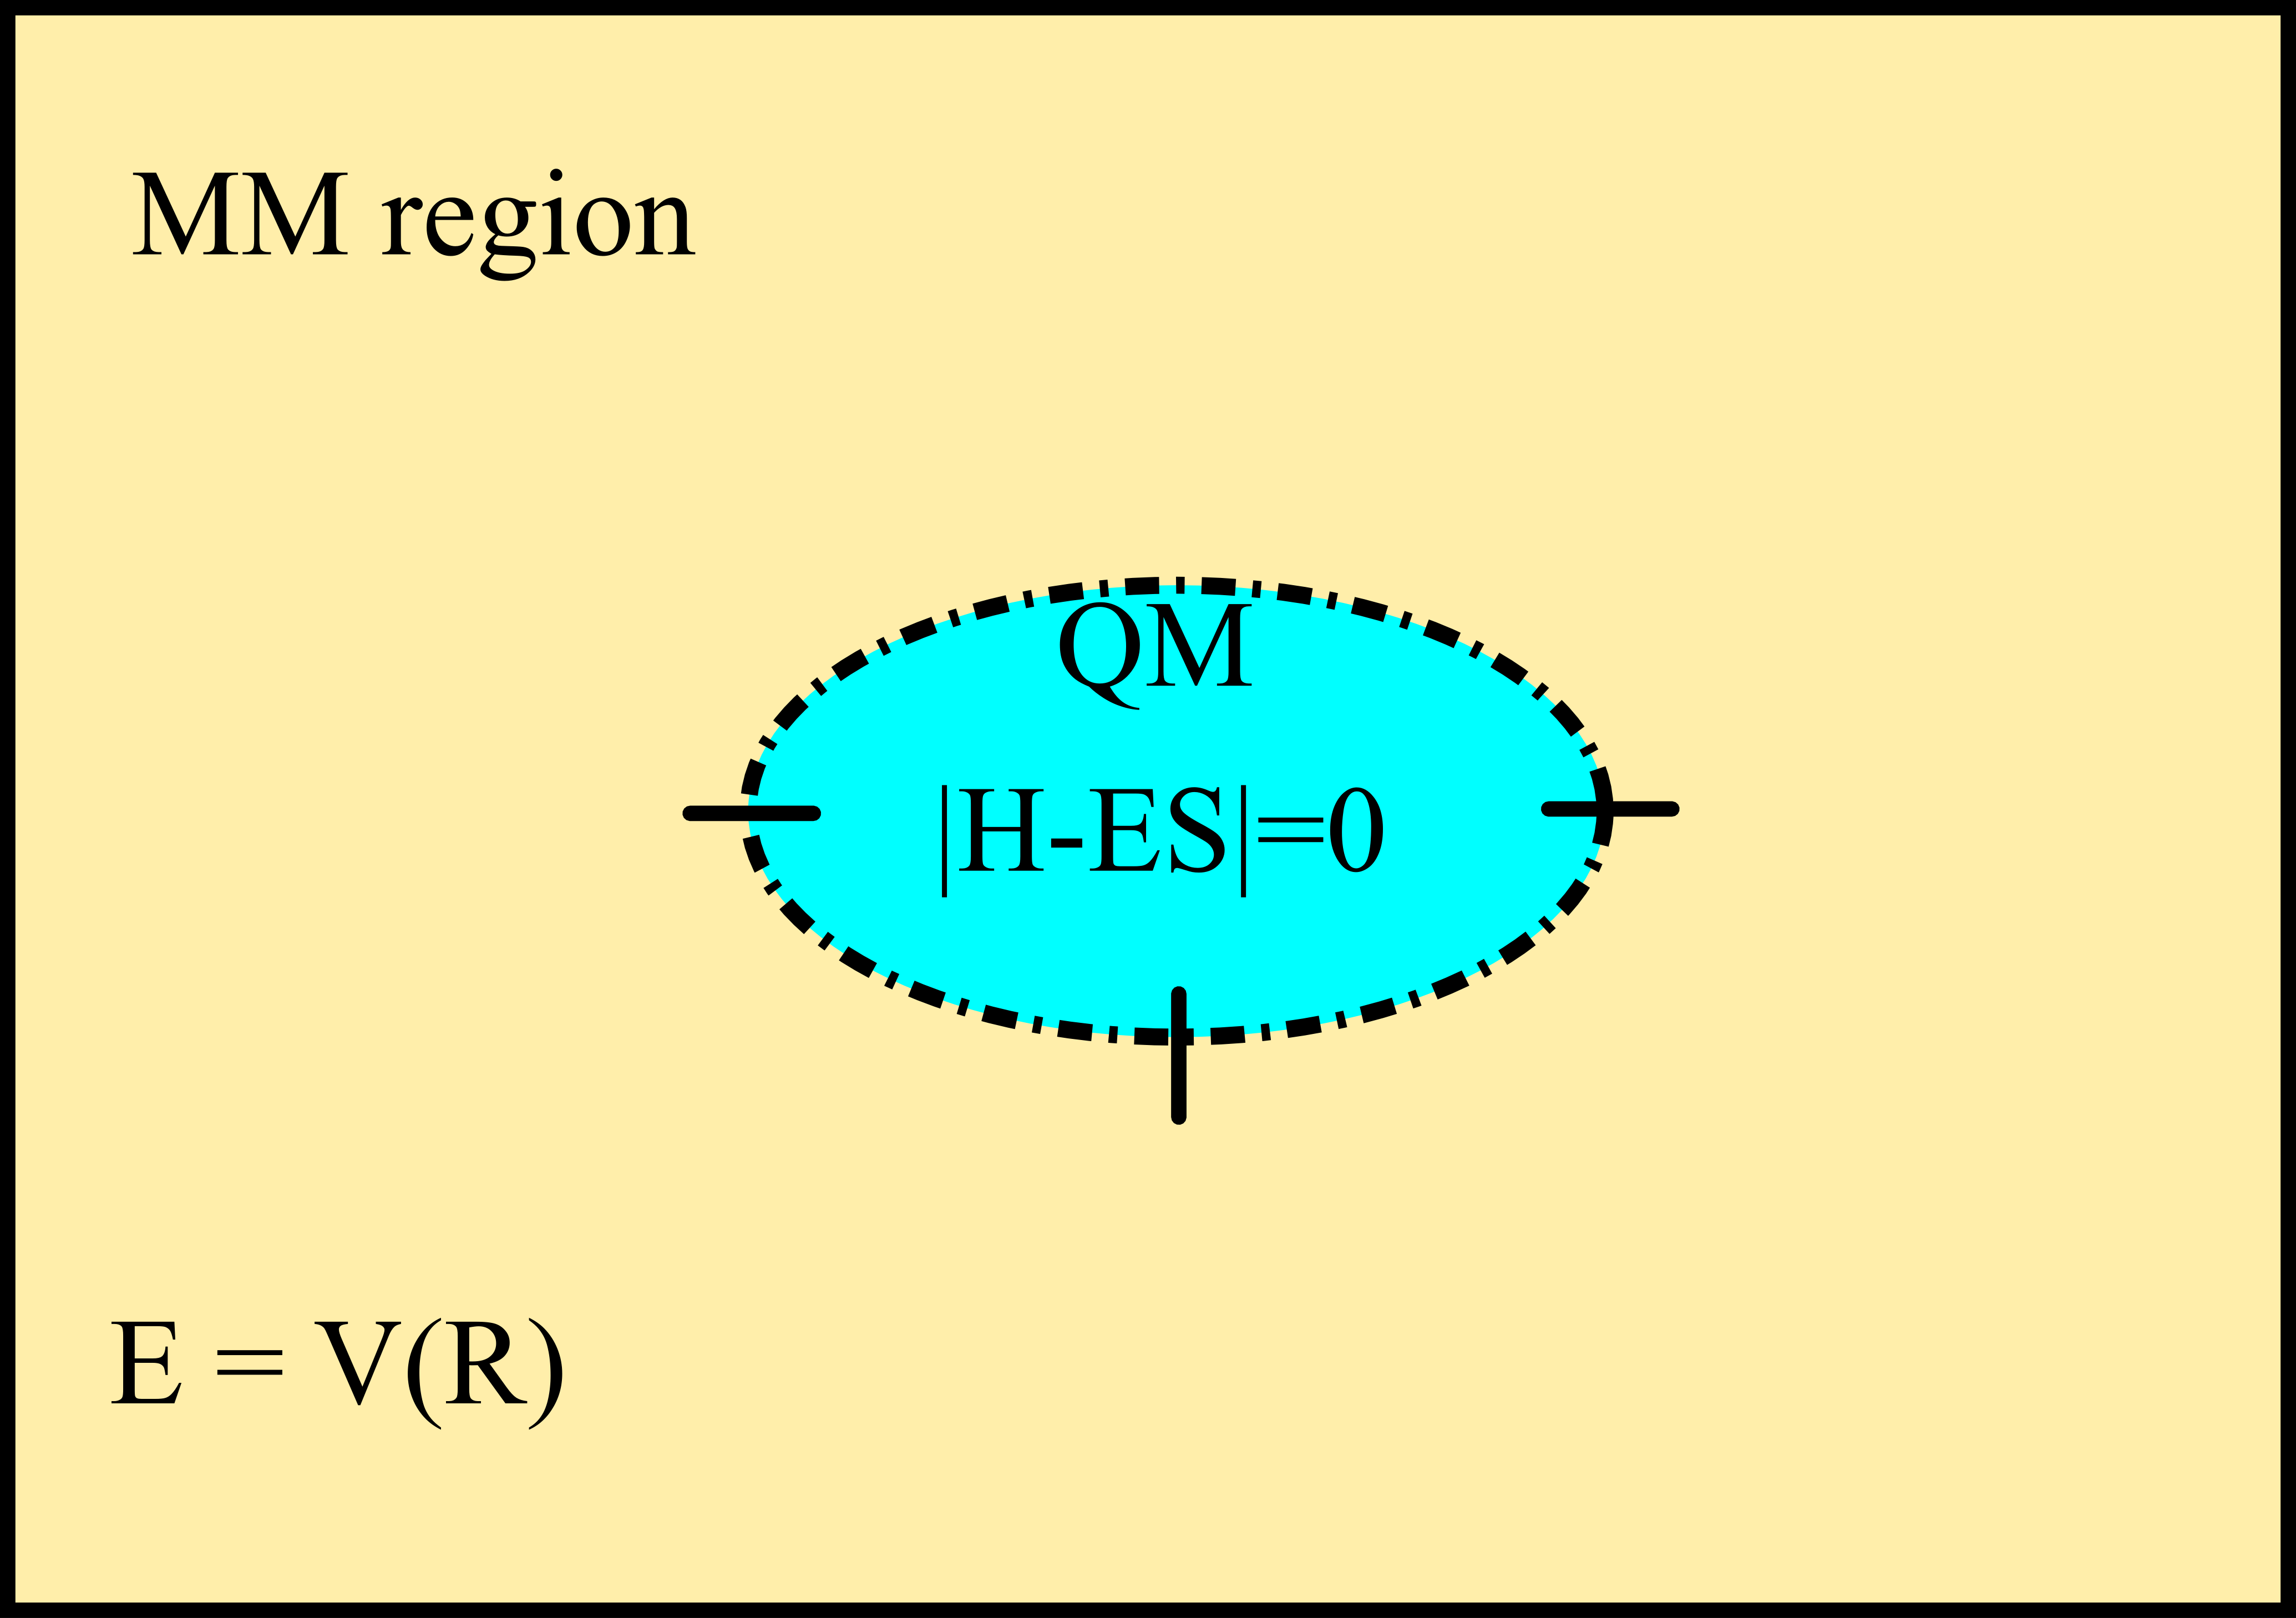
\includegraphics[scale=0.50]{../doc/images/QMMM_1.png}
 \caption{Schematic of a QMMM simulation box with bonds between the QM and MM
 regions.}
 \label{fig:QMMM1}
\end{figure}

QMMM calculations divide the system into regions which require accurate
quantum treatment and regions that can safely be approximated by classical
models (see Figure \ref{fig:QMMM1}). The full effective Hamiltonian, 
$\hat H_{eff}$, can be written as
\begin{equation}
 \hat H_{eff} = \hat H_{qm} + \hat V_{mm} + \hat V_{qmmm} \; ,
\end{equation}
where $\hat H_{qm}$ is the Hamiltonian for the QM region, $\hat V_{mm}$
is the classical potential for the MM region, and $\hat V_{qmmm}$ is the
potential for the interaction of the QM and MM regions. \\

Since the MM and QMMM interface are included only through the potential,
solving the Schr\"odinger equation is essentially trivial.
\begin{equation}
 E \approx \langle \psi |\hat H_{eff}|\psi \rangle
\end{equation}

\subsection{QM-MM interactions}

When the QM and MM regions are not connected by covalent bonds, the QM-MM
interactions are reasonably straightforward. The interaction between the
electric field of the MM region (point charges or multipoles) and the QM
region is calculated by adding point charges to the QM calculations. This
allows for electrostatic repulsion and polarization, but neglects exchange
and dispersion interactions. These missing interactions are added using the
vdW potentials taken from the MM force field. \\

For a single-point energy, the QM+charges calculation is performed with the QM
wrapper, while the MM wrapper calculates the MM energy with no charges or
bonded potentials on any of the QM atoms. These two energies are then added
together to get the total energy. This approach splits $\hat V_{qmmm}$ between
the MM calculation ($\hat V_{mm}$) and the QM calculation ($\hat H_{qm}$). 

\FloatBarrier

\subsection{Pseudo-bond method}

\begin{figure}[hbt]
 \centering
 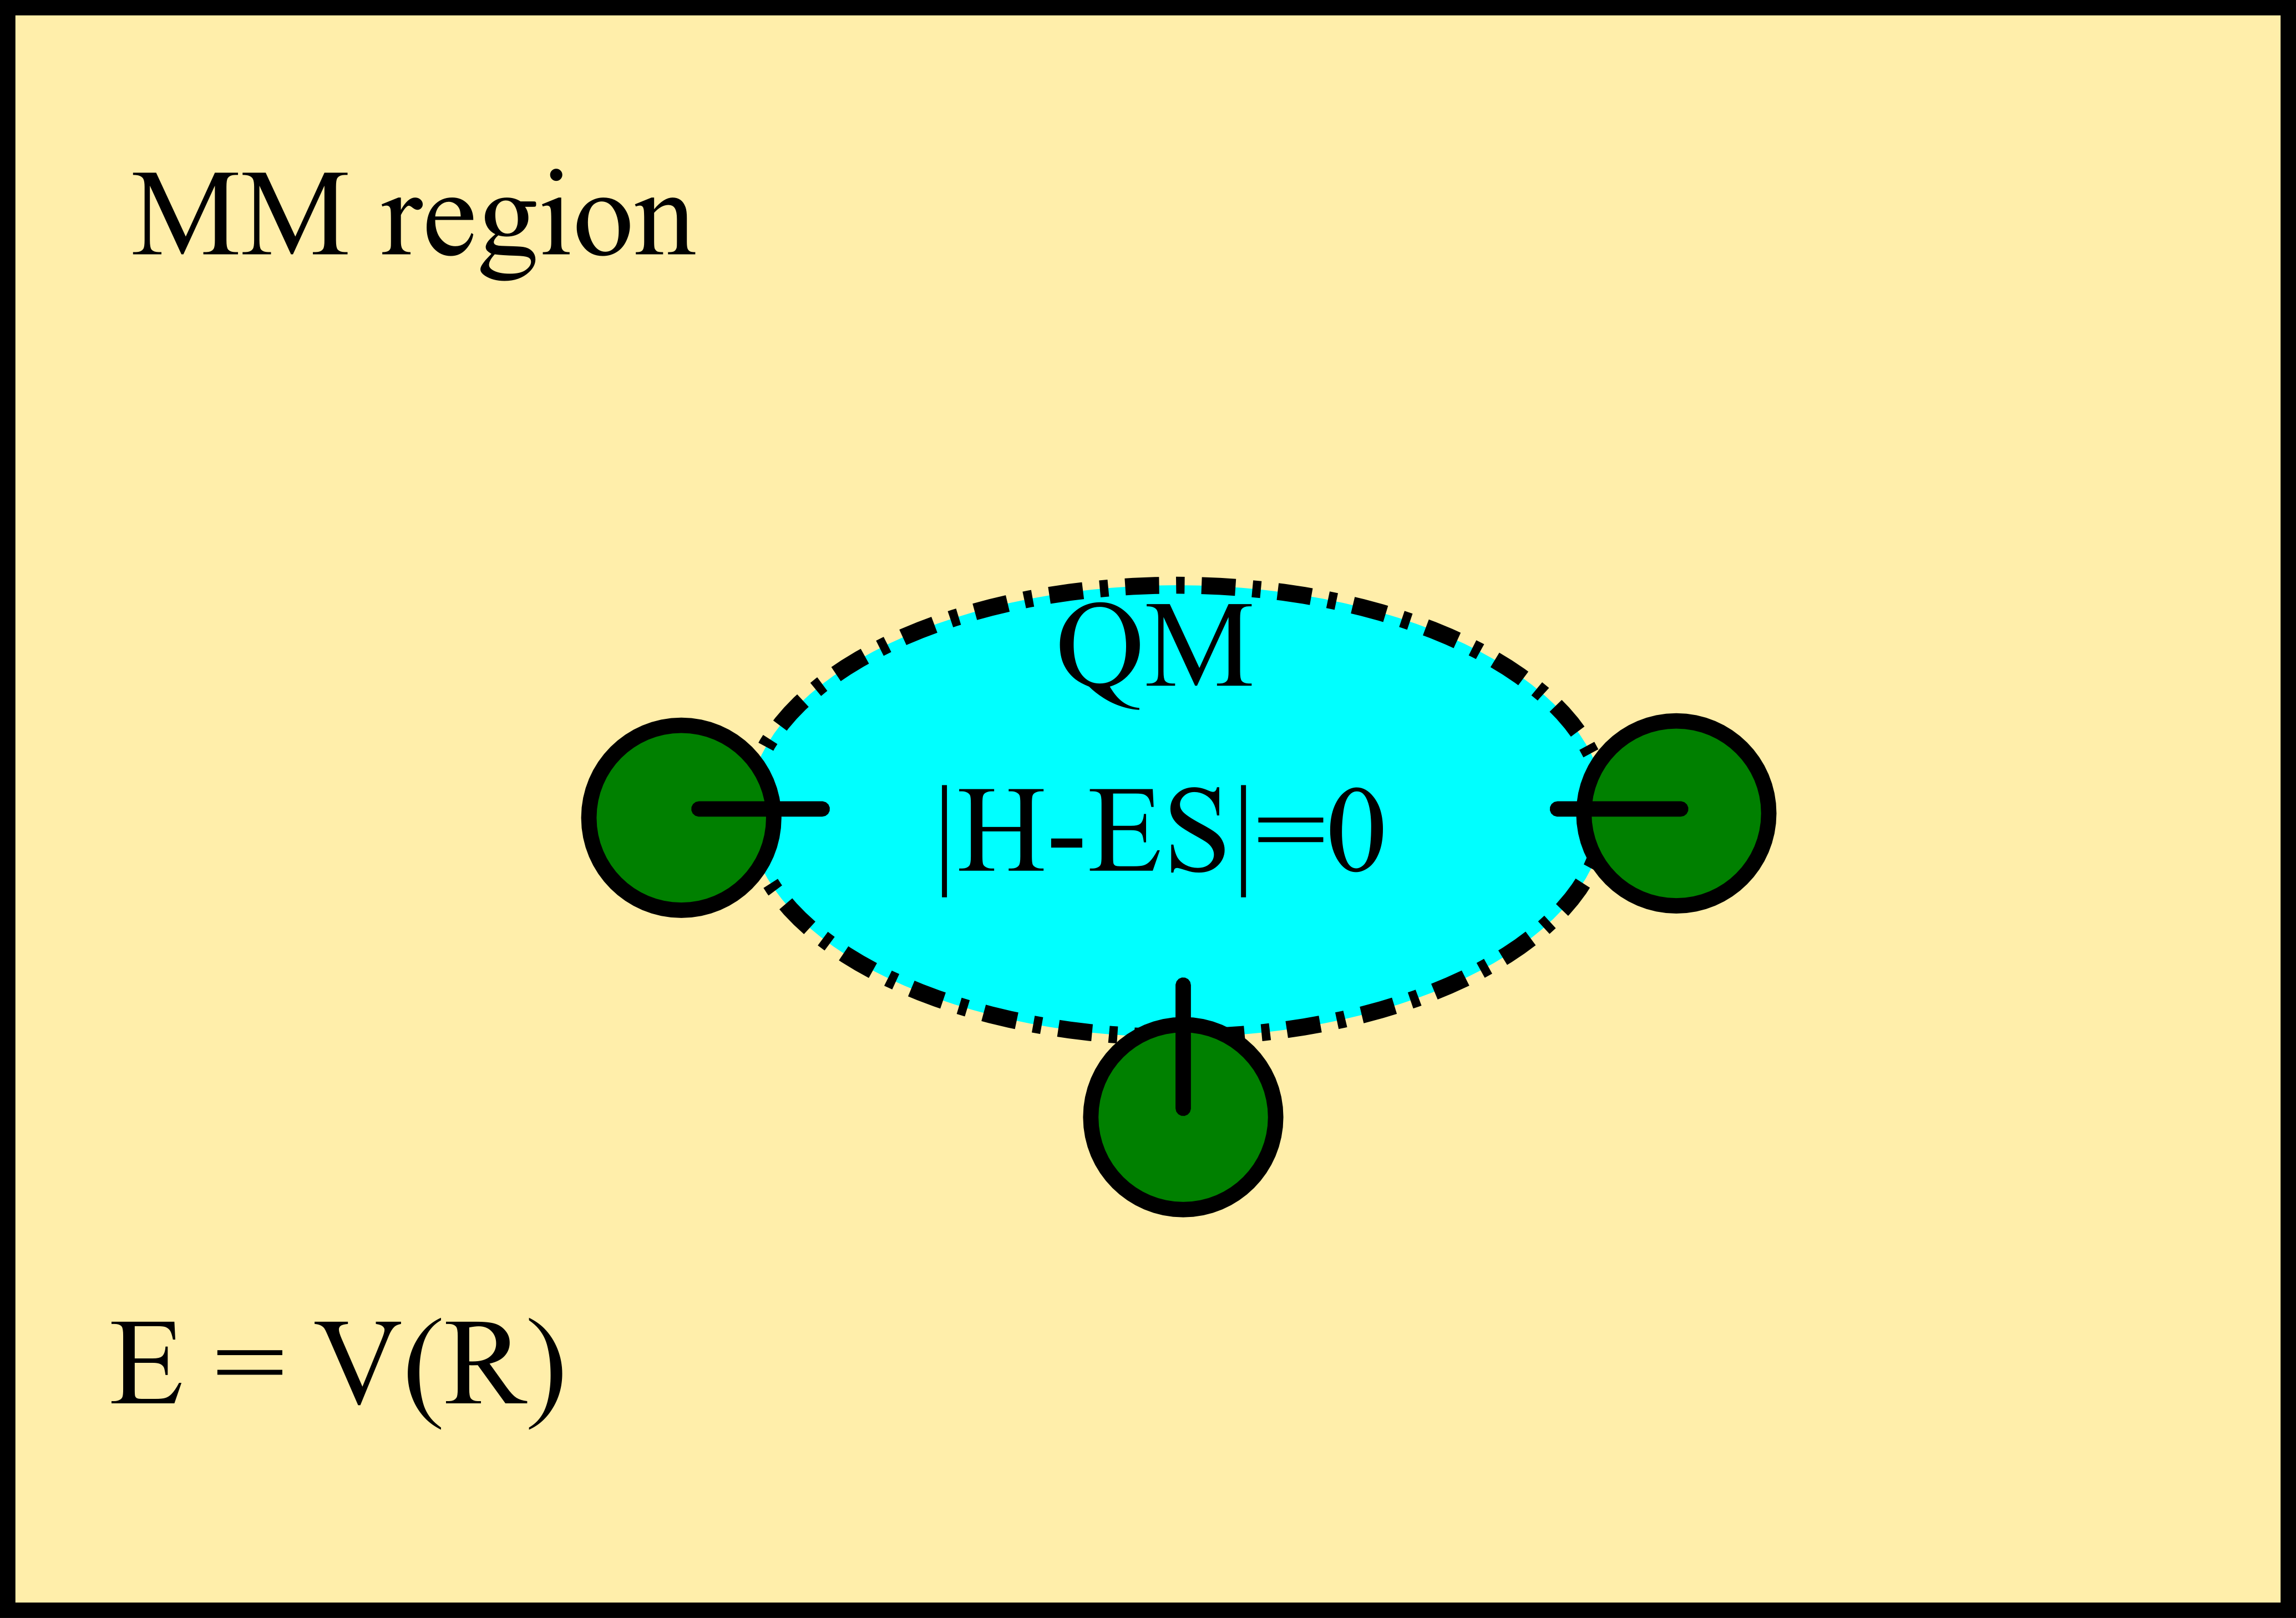
\includegraphics[scale=0.50]{../doc/images/QMMM_2.png}
 \caption{Schematic of a QMMM simulation box with the boundary region shown in
 green between the QM and MM regions.}
 \label{fig:QMMM2}
\end{figure} 

\begin{table}[hbt]
 \centering
 \begin{tabular}{|c|c c|}
 \hline
  & \multicolumn{2}{|c|}{Wrapper calculation} \\
 Int. type & MM & QM \\ \hline
 MM-MM & FF & Zero \\
 QM-QM & Zero & $\rho_{el}$ \\
 PA-PA & FF & PP+$\rho_{el}$ \\
 BA-BA & FF & Zero \\
 QM-MM & FF-\{$q_{qm}$\} & $\rho_{el}$+\{$q_{mm}$\} \\
 QM-PA & Bonds & PP+$\rho_{el}$ \\
 QM-BA & FF-\{$q_{qm}$\} & Zero \\
 MM-PA & FF & PP+$\rho_{el}$+\{$q_{mm}$\} \\
 MM-BA & FF & Zero \\
 PA-BA & FF & Zero \\ \hline
 \end{tabular}
 \caption{The treatment of region-region interactions in the MM and QM 
 wrappers during single-point energy calculations. Interactions were 
 abbreviated as follows: force field (FF), electron density ($\rho_{el}$),
 pseudopotential (PP), no interaction (Zero), QM point charges 
 (\{$q_{qm}$\}), MM bond potentials (Bonds), and MM point charges
 (\{$q_{mm}$\}). A "-" sign is used if the interaction is removed instead of
 added (i.e. FF-\{$q_{qm}$\} denotes the force field with no charges on the
 QM atoms).} 
 \label{tab:IntTable}
\end{table}

\begin{figure}[hbt]
 \centering  
 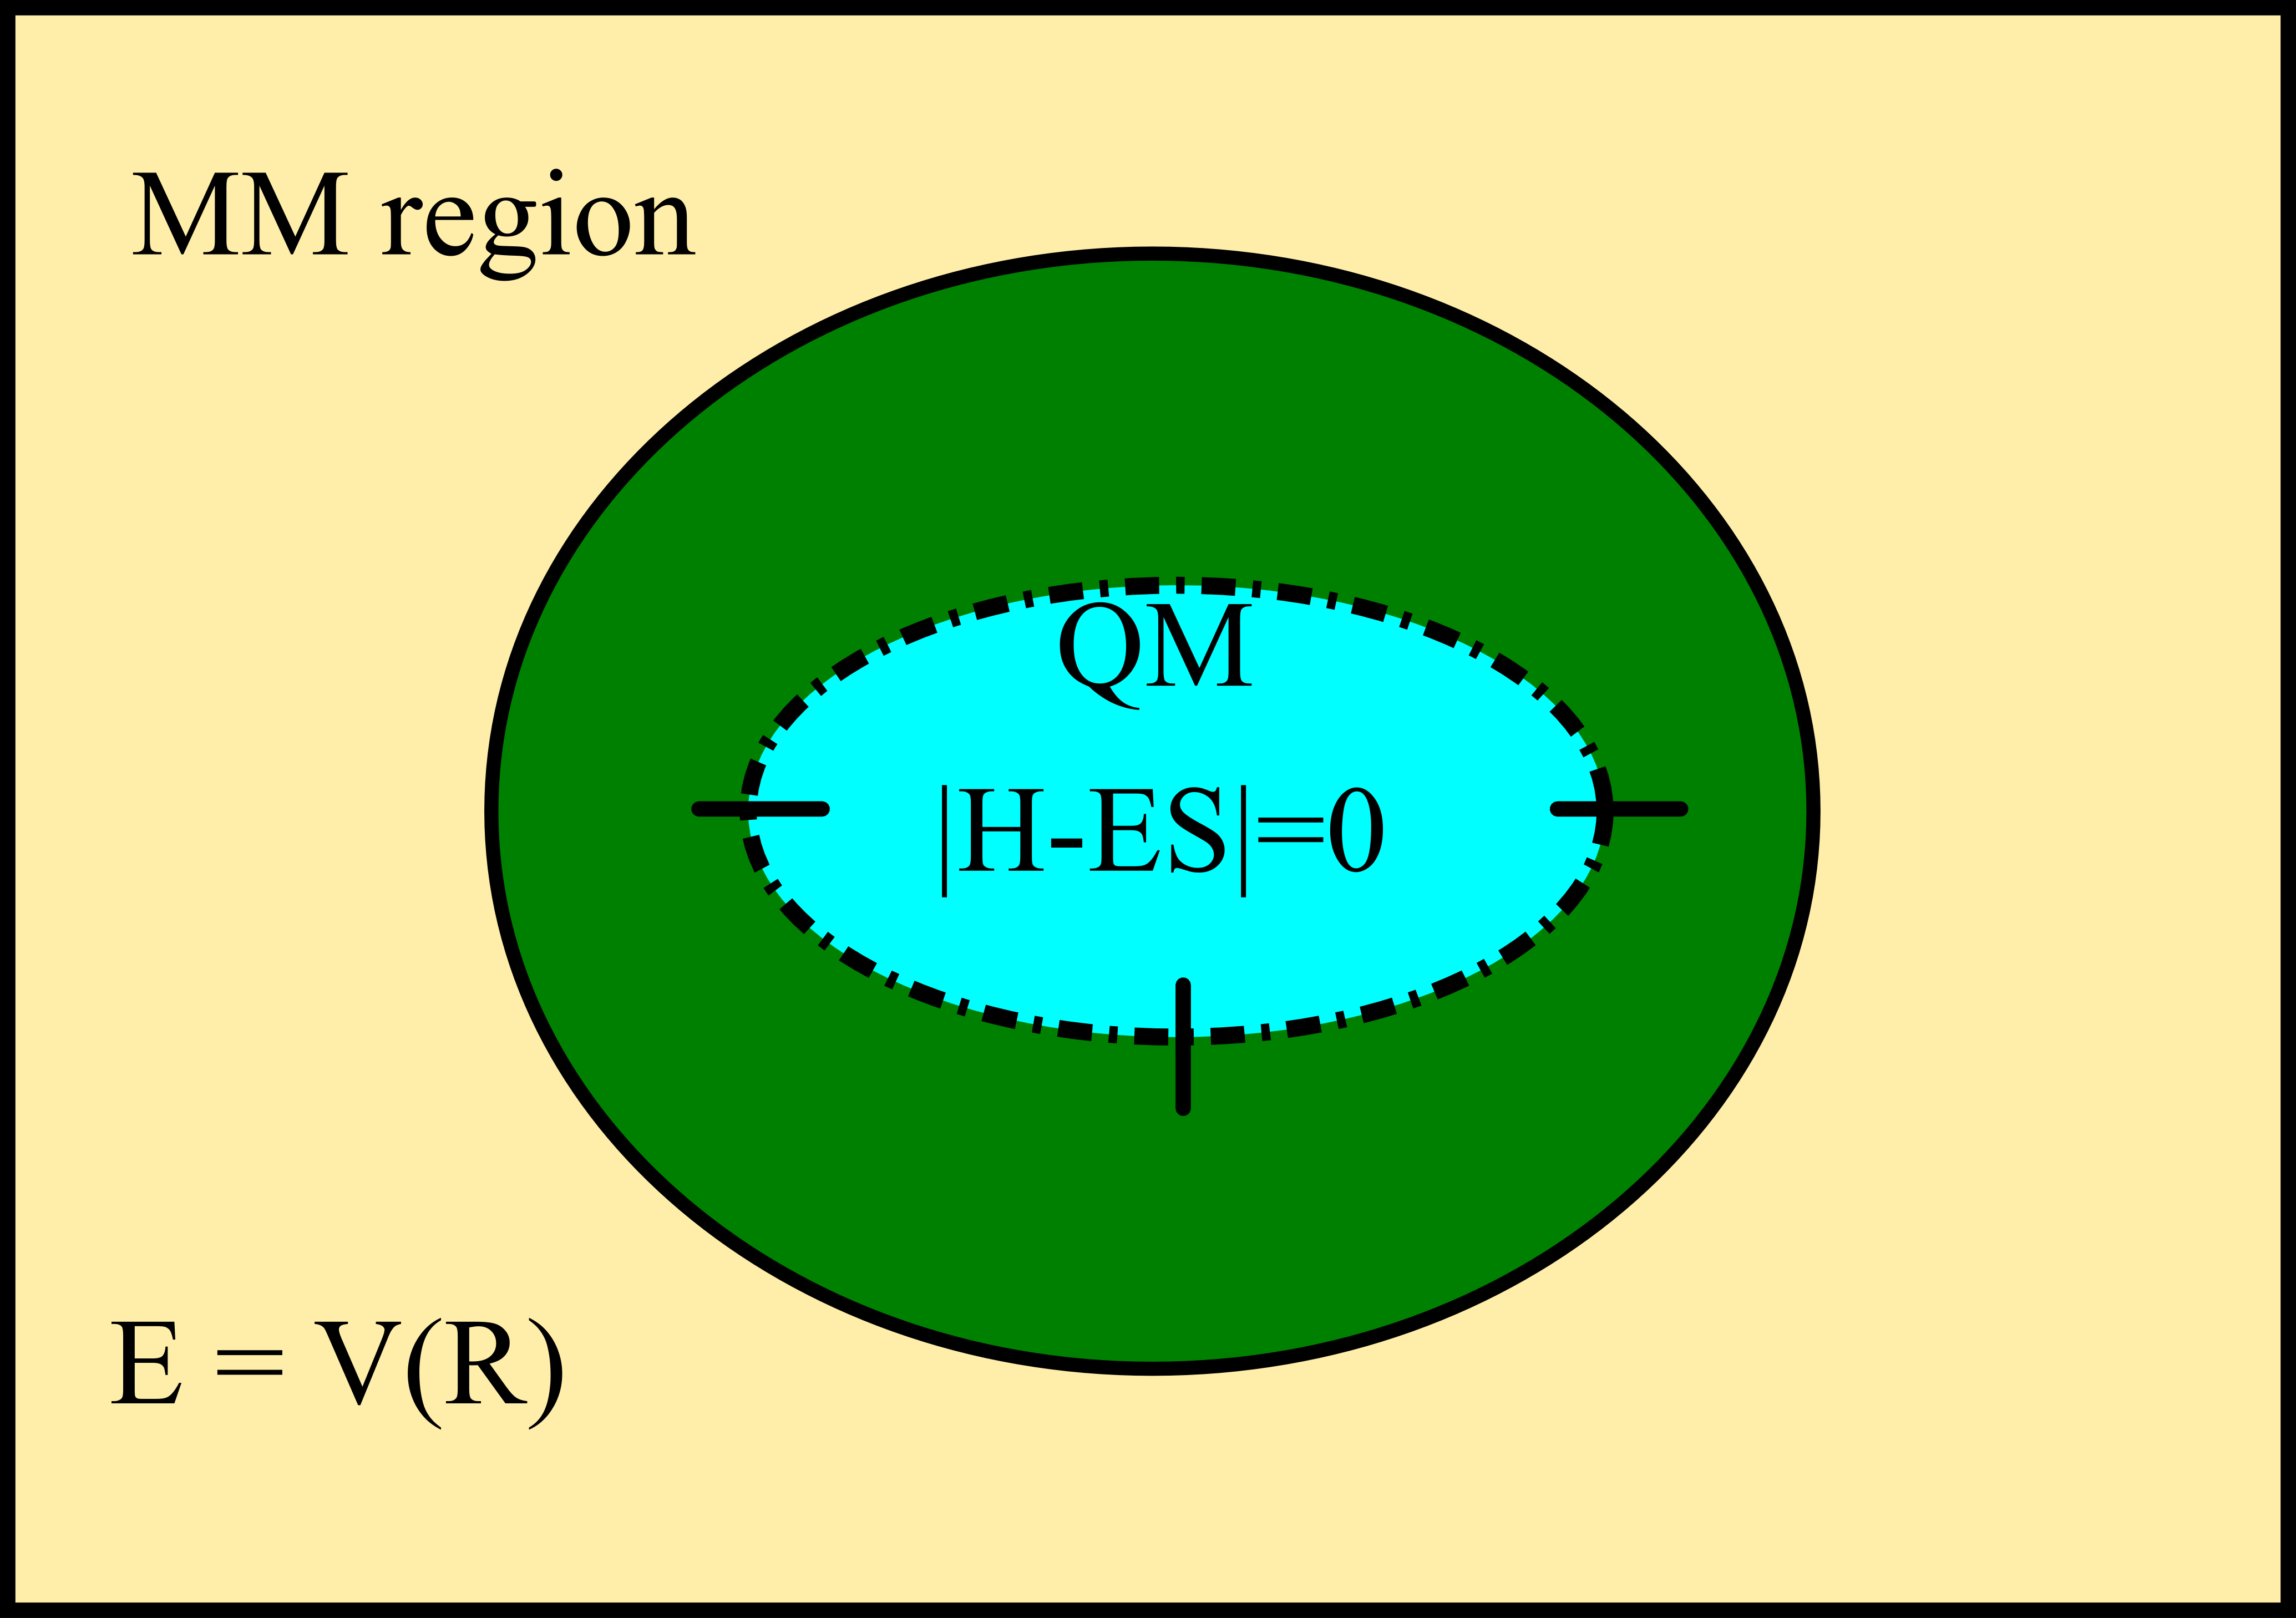
\includegraphics[scale=0.50]{../doc/images/QMMM_3.png}
 \caption{Schematic of a QMMM simulation box with a large boundary region
 between the QM and MM regions.}
 \label{fig:QMMM3}
\end{figure}

The calculations are more complicated when there are bonds between the QM and
MM regions. Covalent bonds require two additional regions of the QMMM system,
a pseudo-atom (PA) region and a boundary atom (BA) region. Pseudo-atoms are
shared by the QM and MM regions, and handle the bulk of the covalent
interactions. The severed bonds from the MM region are treated by adding a
pseudopotential to the pseudo-atoms that allows a fluorine atom to mimic the
behavior of an sp$^3$ hybridized carbon or nitrogen atom. Boundary atoms
correct for two additional errors. First, having point charges close to the
QM region can cause the electron density to be over-polarized. The second
error is introduced by the fact that the QM region must have an integer number
of electrons. Both of these problems can be mitigated by absorbing the point
charges on the atoms bonded to the pseudo-atoms into the QM region during the
QM calculation. This produces atoms with zero-charge on the boundaries between
the QM and MM regions. \\

For the MM part of the calculation, the pseudo-atoms and boundary atoms retain
their force field charges, and the MM bonding interactions are added for the
pseudo-atoms. The treatment of different interaction types are given in Table
\ref{tab:IntTable} for single-point energy calculations. In the pseudo-bond
approach, only some of the bonded interactions are calculated for the QMMM
interface. Further detials on which bonded interactions are included can be
found in the literature. \\

So far we have discussed systems similar to the one shown in Figure
\ref{fig:QMMM2}, where the boundary atoms only surround the covalent bonds.
This is due to the primitive treatment of the QM-MM boundaries. A more
complicated scheme can be employed where the boundary atoms are represented by
a polarizable frozen density force field. The QM and frozen density
interactions are more natural than interactions between the QM and point
charges, and thus, this approach avoids the over-polarization. Boundary atoms
represented by frozen electron density can be extended further from the QM
region and can create smoother boundaries between the QM and MM regions.
Ideally, a system could be constructed with a large boundary region between
the QM and MM regions (see Figure \ref{fig:QMMM3}).

\FloatBarrier

\section{Monte Carlo Simulations}

\subsection{Stochastic sampling}

Monte Carlo simulations sample phase space by generation random changes to
the system. Completely random sampling could eventually find a global
minimum, however, majority of the random structures would have energies well
above $kT$ and contribute very little to the statistical averages. \\

Almost any type of change can be made to the system in a Monte Carlo
simulation. The primary limitations are the creativity of the programmer and
the efficiency of making the changes. This allows Monte Carlo simulations to
be tailored to the system and focus on the randomly changing the most important 
features of a system. \\

If the moving atoms and/or type of random change are chosen randomly, this
procedure satisfies "detailed balance." I.e. the move from configuration $i$
to configuration $j$ can be reversed by a move from configuration $j$ to
configuration $i$.

\subsection{Canonical ensemble}

A more efficient approach is to accept or reject the random moves based on
the Boltzmann weight of the configuration.
\begin{equation}
 P_{acc} \propto e^{-\Delta E\beta} \; ,
\end{equation}
where $P_{acc}$ is the probability of accepting the move, $\Delta E$ is the 
change in energy, and $\beta$ is the inverse temperature,
\begin{equation} 
 \beta = \frac{1}{kT} \; .
\end{equation}
This proceedure leads to biased sampling of the lower energy states. \\

Unlike molecular dynamics simulations, the natural ensemble for Monte Carlo
simulations is the canonical ensemble (NVT). This is advantageous since there
is no need to couple the simulation to a thermostat.

\subsection{Isobaric-isothermal ensemble}

Although NVT simulations are natural for Monte Carlo, it is relatively easy to
change to the NPT ensemble. NPT simulations are performed by randomly changing
the volume of the simulation box. This procedure produces a slightly
different expression for the probabilities,
\begin{equation}
 P_{acc} \propto e^{-(P\Delta V+\Delta E)\beta+N\Delta ln(V)} \; ,
\end{equation}
where $P$ is the pressure, $\Delta V$ is the change in volume, and $N$ is
the number of atoms.

\FloatBarrier

\section{Path-Integral Monte Carlo}

\subsection{Path-integral formalism}



\subsection{PIMC simulations}

Path-integral Monte Carlo simulations are performed by simulating a large
number of classical systems which are then coupled together via harmonic
bonds. Allowed Monte Carlo moves include displacements of single beads,
translations of centroids, and changes of the volume.

The spring energy between the beads represents the quantum kinetic energy of
the centroid. Moves are accepted based on the effective energy, $E_{eff}$
\begin{equation}
 E_{eff} = E_{spring}+\frac{1}{N_p}\sum_i^{N_p} E_{pot,i} \; ,
\end{equation}
where the spring energy is given by
\begin{equation}
 E_{spring} = \sum_{j}^{N_a} \frac{m_{j}N_{p}}{\hbar^2\beta^2}
              \sum_{i}^{N_p} (r_{i}-r_{i-1})^2  \; .
\end{equation}
Here the $N_a$ is the total number of atoms, $N_p$ is the number of beads,
$r_i$ is the position of bead $i$, and $E_{pot}$ is the potential energy. The
acceptance probability is given by
\begin{equation}
 P_{acc} \propto e^{\Delta E_{eff}\beta} \; .
\end{equation}

The path-integral total energy is slightly different from the effective
potential.
\begin{equation}
 \label{eq:pitotal}
 E_{pi} = \frac{3N_aN_p}{2\beta}-E_{spring}
          +\frac{1}{N_p}\sum_i^{N_p} E_{pot,i} \; ,
\end{equation}
where $E_{pi}$ is the total energy. The first two terms in Eq.\
\ref{eq:pitotal} represent the classical kinetic energy for all particles and
the amount of kinetic energy absorbed by centroid harmonic bonds.

\subsection{Ergodicity}

Classical Monte Carlo simulations typically scale as $N_a^2$ due to the
pairwise force field interactions of the atoms. Since path-integral
simulations have $N_p$ simulations that run in tandem, the overall scaling is
$N_pN_a^2$. In addition to making the energy calculations computationally more
expensive, the efficiencies of the Monte Carlo moves tend to decrease. Monte
Carlo moves typically consist of changes to the positions of a single atom or
possibly more complicated moves where bond angles are shifted. This leads to
large systems changing very slowly and the path-integral formalism essentially
increases the size of the system. \\

Another problem introduced by the path-integral formalism comes from the
harmonic constraints between the beads. The force constants for the
path-integral springs is proportional to the mass of the particle, which means
that heavy atoms can experience very strong forces holding the centroid
close together. The presence of strong potentials restricts the movement of
the atoms, and reduces $P_{acc}$.

\FloatBarrier
\bibliographystyle{unsrt}
\bibliography{../manual.bib}

\end{document}
